% Created by tikzDevice version 0.12.3.1 on 2022-03-13 08:38:22
% !TEX encoding = UTF-8 Unicode
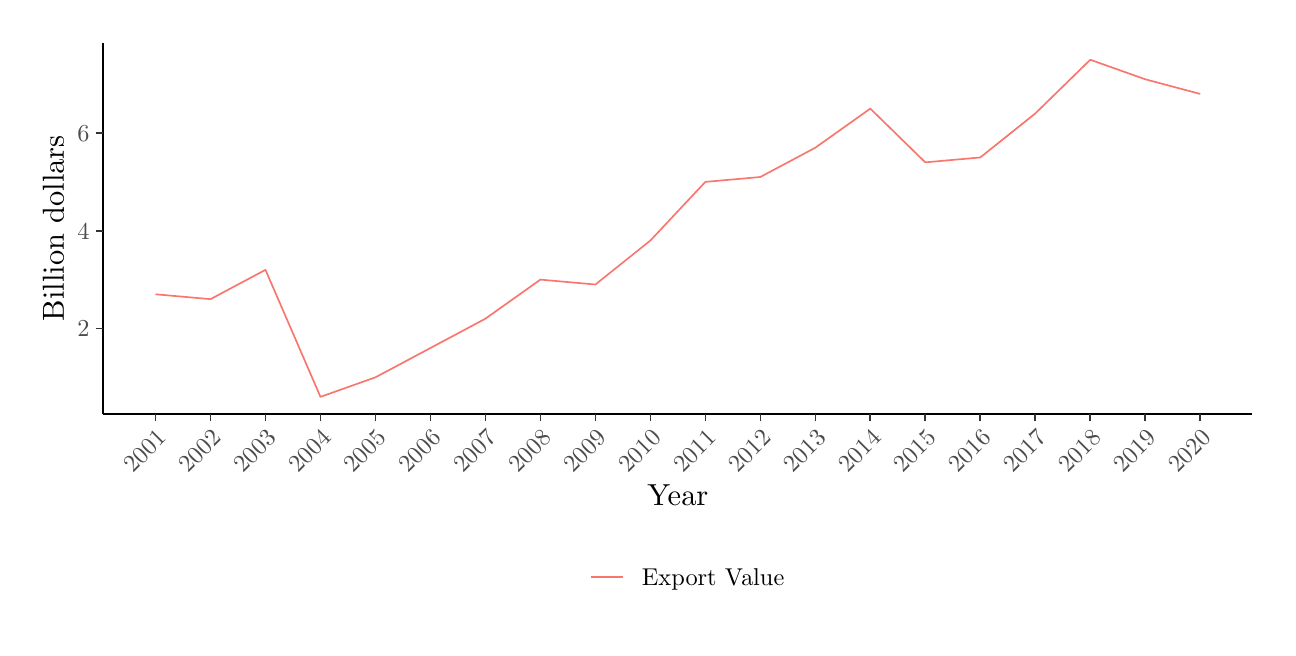
\begin{tikzpicture}[x=1pt,y=1pt]
\definecolor{fillColor}{RGB}{255,255,255}
\path[use as bounding box,fill=fillColor,fill opacity=0.00] (0,0) rectangle (448.07,216.81);
\begin{scope}
\path[clip] (  0.00,  0.00) rectangle (448.07,216.81);
\definecolor{drawColor}{RGB}{255,255,255}
\definecolor{fillColor}{RGB}{255,255,255}

\path[draw=drawColor,line width= 0.6pt,line join=round,line cap=round,fill=fillColor] (  0.00,  0.00) rectangle (448.07,216.81);
\end{scope}
\begin{scope}
\path[clip] ( 27.31, 77.31) rectangle (442.57,211.31);
\definecolor{fillColor}{RGB}{255,255,255}

\path[fill=fillColor] ( 27.31, 77.31) rectangle (442.57,211.31);
\definecolor{drawColor}{RGB}{248,118,109}

\path[draw=drawColor,line width= 0.6pt,line join=round] ( 46.19,120.47) --
	( 66.06,118.71) --
	( 85.93,129.30) --
	(105.80, 83.40) --
	(125.66, 90.46) --
	(145.53,101.05) --
	(165.40,111.65) --
	(185.27,125.77) --
	(205.14,124.00) --
	(225.01,139.89) --
	(244.88,161.08) --
	(264.75,162.85) --
	(284.62,173.44) --
	(304.48,187.56) --
	(324.35,168.14) --
	(344.22,169.91) --
	(364.09,185.80) --
	(383.96,205.22) --
	(403.83,198.16) --
	(423.70,192.86);
\end{scope}
\begin{scope}
\path[clip] (  0.00,  0.00) rectangle (448.07,216.81);
\definecolor{drawColor}{RGB}{0,0,0}

\path[draw=drawColor,line width= 0.6pt,line join=round] ( 27.31, 77.31) --
	( 27.31,211.31);
\end{scope}
\begin{scope}
\path[clip] (  0.00,  0.00) rectangle (448.07,216.81);
\definecolor{drawColor}{gray}{0.30}

\node[text=drawColor,anchor=base east,inner sep=0pt, outer sep=0pt, scale=  0.88] at ( 22.36,105.08) {2};

\node[text=drawColor,anchor=base east,inner sep=0pt, outer sep=0pt, scale=  0.88] at ( 22.36,140.39) {4};

\node[text=drawColor,anchor=base east,inner sep=0pt, outer sep=0pt, scale=  0.88] at ( 22.36,175.71) {6};
\end{scope}
\begin{scope}
\path[clip] (  0.00,  0.00) rectangle (448.07,216.81);
\definecolor{drawColor}{gray}{0.20}

\path[draw=drawColor,line width= 0.6pt,line join=round] ( 24.56,108.11) --
	( 27.31,108.11);

\path[draw=drawColor,line width= 0.6pt,line join=round] ( 24.56,143.43) --
	( 27.31,143.43);

\path[draw=drawColor,line width= 0.6pt,line join=round] ( 24.56,178.74) --
	( 27.31,178.74);
\end{scope}
\begin{scope}
\path[clip] (  0.00,  0.00) rectangle (448.07,216.81);
\definecolor{drawColor}{RGB}{0,0,0}

\path[draw=drawColor,line width= 0.6pt,line join=round] ( 27.31, 77.31) --
	(442.57, 77.31);
\end{scope}
\begin{scope}
\path[clip] (  0.00,  0.00) rectangle (448.07,216.81);
\definecolor{drawColor}{gray}{0.20}

\path[draw=drawColor,line width= 0.6pt,line join=round] ( 46.19, 74.56) --
	( 46.19, 77.31);

\path[draw=drawColor,line width= 0.6pt,line join=round] ( 66.06, 74.56) --
	( 66.06, 77.31);

\path[draw=drawColor,line width= 0.6pt,line join=round] ( 85.93, 74.56) --
	( 85.93, 77.31);

\path[draw=drawColor,line width= 0.6pt,line join=round] (105.80, 74.56) --
	(105.80, 77.31);

\path[draw=drawColor,line width= 0.6pt,line join=round] (125.66, 74.56) --
	(125.66, 77.31);

\path[draw=drawColor,line width= 0.6pt,line join=round] (145.53, 74.56) --
	(145.53, 77.31);

\path[draw=drawColor,line width= 0.6pt,line join=round] (165.40, 74.56) --
	(165.40, 77.31);

\path[draw=drawColor,line width= 0.6pt,line join=round] (185.27, 74.56) --
	(185.27, 77.31);

\path[draw=drawColor,line width= 0.6pt,line join=round] (205.14, 74.56) --
	(205.14, 77.31);

\path[draw=drawColor,line width= 0.6pt,line join=round] (225.01, 74.56) --
	(225.01, 77.31);

\path[draw=drawColor,line width= 0.6pt,line join=round] (244.88, 74.56) --
	(244.88, 77.31);

\path[draw=drawColor,line width= 0.6pt,line join=round] (264.75, 74.56) --
	(264.75, 77.31);

\path[draw=drawColor,line width= 0.6pt,line join=round] (284.62, 74.56) --
	(284.62, 77.31);

\path[draw=drawColor,line width= 0.6pt,line join=round] (304.48, 74.56) --
	(304.48, 77.31);

\path[draw=drawColor,line width= 0.6pt,line join=round] (324.35, 74.56) --
	(324.35, 77.31);

\path[draw=drawColor,line width= 0.6pt,line join=round] (344.22, 74.56) --
	(344.22, 77.31);

\path[draw=drawColor,line width= 0.6pt,line join=round] (364.09, 74.56) --
	(364.09, 77.31);

\path[draw=drawColor,line width= 0.6pt,line join=round] (383.96, 74.56) --
	(383.96, 77.31);

\path[draw=drawColor,line width= 0.6pt,line join=round] (403.83, 74.56) --
	(403.83, 77.31);

\path[draw=drawColor,line width= 0.6pt,line join=round] (423.70, 74.56) --
	(423.70, 77.31);
\end{scope}
\begin{scope}
\path[clip] (  0.00,  0.00) rectangle (448.07,216.81);
\definecolor{drawColor}{gray}{0.30}

\node[text=drawColor,rotate= 45.00,anchor=base east,inner sep=0pt, outer sep=0pt, scale=  0.88] at ( 50.47, 68.07) {2001};

\node[text=drawColor,rotate= 45.00,anchor=base east,inner sep=0pt, outer sep=0pt, scale=  0.88] at ( 70.34, 68.07) {2002};

\node[text=drawColor,rotate= 45.00,anchor=base east,inner sep=0pt, outer sep=0pt, scale=  0.88] at ( 90.21, 68.07) {2003};

\node[text=drawColor,rotate= 45.00,anchor=base east,inner sep=0pt, outer sep=0pt, scale=  0.88] at (110.08, 68.07) {2004};

\node[text=drawColor,rotate= 45.00,anchor=base east,inner sep=0pt, outer sep=0pt, scale=  0.88] at (129.95, 68.07) {2005};

\node[text=drawColor,rotate= 45.00,anchor=base east,inner sep=0pt, outer sep=0pt, scale=  0.88] at (149.82, 68.07) {2006};

\node[text=drawColor,rotate= 45.00,anchor=base east,inner sep=0pt, outer sep=0pt, scale=  0.88] at (169.69, 68.07) {2007};

\node[text=drawColor,rotate= 45.00,anchor=base east,inner sep=0pt, outer sep=0pt, scale=  0.88] at (189.56, 68.07) {2008};

\node[text=drawColor,rotate= 45.00,anchor=base east,inner sep=0pt, outer sep=0pt, scale=  0.88] at (209.43, 68.07) {2009};

\node[text=drawColor,rotate= 45.00,anchor=base east,inner sep=0pt, outer sep=0pt, scale=  0.88] at (229.29, 68.07) {2010};

\node[text=drawColor,rotate= 45.00,anchor=base east,inner sep=0pt, outer sep=0pt, scale=  0.88] at (249.16, 68.07) {2011};

\node[text=drawColor,rotate= 45.00,anchor=base east,inner sep=0pt, outer sep=0pt, scale=  0.88] at (269.03, 68.07) {2012};

\node[text=drawColor,rotate= 45.00,anchor=base east,inner sep=0pt, outer sep=0pt, scale=  0.88] at (288.90, 68.07) {2013};

\node[text=drawColor,rotate= 45.00,anchor=base east,inner sep=0pt, outer sep=0pt, scale=  0.88] at (308.77, 68.07) {2014};

\node[text=drawColor,rotate= 45.00,anchor=base east,inner sep=0pt, outer sep=0pt, scale=  0.88] at (328.64, 68.07) {2015};

\node[text=drawColor,rotate= 45.00,anchor=base east,inner sep=0pt, outer sep=0pt, scale=  0.88] at (348.51, 68.07) {2016};

\node[text=drawColor,rotate= 45.00,anchor=base east,inner sep=0pt, outer sep=0pt, scale=  0.88] at (368.38, 68.07) {2017};

\node[text=drawColor,rotate= 45.00,anchor=base east,inner sep=0pt, outer sep=0pt, scale=  0.88] at (388.25, 68.07) {2018};

\node[text=drawColor,rotate= 45.00,anchor=base east,inner sep=0pt, outer sep=0pt, scale=  0.88] at (408.12, 68.07) {2019};

\node[text=drawColor,rotate= 45.00,anchor=base east,inner sep=0pt, outer sep=0pt, scale=  0.88] at (427.98, 68.07) {2020};
\end{scope}
\begin{scope}
\path[clip] (  0.00,  0.00) rectangle (448.07,216.81);
\definecolor{drawColor}{RGB}{0,0,0}

\node[text=drawColor,anchor=base,inner sep=0pt, outer sep=0pt, scale=  1.10] at (234.94, 44.09) {Year};
\end{scope}
\begin{scope}
\path[clip] (  0.00,  0.00) rectangle (448.07,216.81);
\definecolor{drawColor}{RGB}{0,0,0}

\node[text=drawColor,rotate= 90.00,anchor=base,inner sep=0pt, outer sep=0pt, scale=  1.10] at ( 13.08,144.31) {Billion dollars};
\end{scope}
\begin{scope}
\path[clip] (  0.00,  0.00) rectangle (448.07,216.81);
\definecolor{fillColor}{RGB}{255,255,255}

\path[fill=fillColor] (190.98,  5.50) rectangle (278.90, 30.95);
\end{scope}
\begin{scope}
\path[clip] (  0.00,  0.00) rectangle (448.07,216.81);
\definecolor{drawColor}{RGB}{248,118,109}

\path[draw=drawColor,line width= 0.6pt,line join=round] (203.43, 18.23) -- (214.99, 18.23);
\end{scope}
\begin{scope}
\path[clip] (  0.00,  0.00) rectangle (448.07,216.81);
\definecolor{drawColor}{RGB}{0,0,0}

\node[text=drawColor,anchor=base west,inner sep=0pt, outer sep=0pt, scale=  0.88] at (221.94, 15.20) {Export Value};
\end{scope}
\end{tikzpicture}
